\chapter{Proposed Solution}\label{chap:problemsolution}

In this chapter a description about the methodology to approach the problem presented in section \ref{sec:problemstatement_goals} will be made, as well as the architecture designed to the proposed solution and the different modules which composed it.

\section{Methodology}

Once the problem to be solved has a scope of data analysis, in this case unstructured data like texts, it makes sense the use of an appropriate methodology for the field of interest.

\begin{figure}
  \centering
    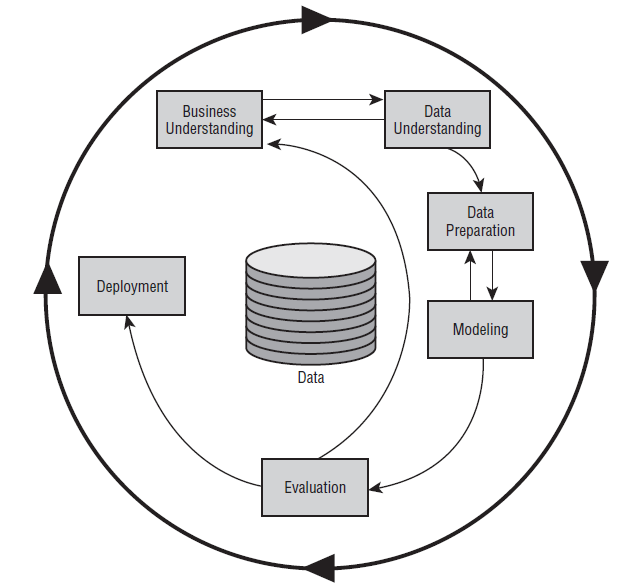
\includegraphics[width=0.7\textwidth]{crisp-dm}
    \caption{CRISP-DM workflow.}
    \label{fig:crisp-dm}
\end{figure}

The CRISP-DM (Cross Industry Standard Process for Data Mining) is the standard model used in the Data Mining field, providing several steps that the specialists may follow to tackle the problem of data analysis. The workflow of this methodology is presented in figure \ref{fig:crisp-dm}. The different model phases are:

\begin{enumerate}
\item \textbf{Business Understanding:} In this phase there are a definition of a work plan and what are the goals to achieve. At this dissertation case, the final goal is to provide a tool capable of helping entities or even ordinary citizens in the decision-making process relatively to some service in the city.
\item \textbf{Data Understanding:} The collection of the dataset is made in this phase as well as the identification of interesting patterns in it.

\item \textbf{Data Preparation:} Dataset cleaning and features engineering are made at this phase. The cleaning task in the text mining field can be seen as the removal of some words, the conversion of words to their root form, and the grouping of two or more words because, sometimes, there are mentions of technical terms or even negations (\textit{n-grams}). The features engineering task is more complicate in the text mining field than in data mining. At common data mining analysis, the data is structured but, in texts, the data is unstructured which make more hardly the discovery of relevant features.

\item \textbf{Modeling:} The modeling phase represents the development of models that will be used in the classification tasks. At this point, it's made, also, some tuning parameters to optimize the models and, where appropriate, the returning to the Data Preparation phase in order to find other features.

\item \textbf{Evaluation:} The results given by the developed model may be evaluated is made in this step. To do that, some evaluation metrics are available (e.g. F1 measure, Area Under the ROC curve, Root Mean Squared Error, etc). The results should be good enough in order to achieve the defined objectives. 

\item \textbf{Deployment:} The knowledge acquired by the model must be harnessed and, in this particular case, must be integrated with the rest of the system to take advantages of its functionality.

One of the main advantages of this methodology is the independence it provides for the development of each of the modules that constitute the desired framework. Its last step allows an iterative integration of the developed models in order to produce the final tool.
\end{enumerate}

\section{Framework}

In order to solve the problem described in Chapter \ref{chap:intro}, the proposed solution is the development of a framework whose usability will be directed to companies or even ordinary users and should be able to provide relevant information about a specific study scenario, namely the transportation area of a city.

\subsection{Architecture Design} \label{sec:architecture}

The framework architecture was designed taking into account all the tasks that have to be performed to solve the different points in which the main problem can be decomposed. A visualization of the architecture can be seen in the figure \ref{fig:framework}.

Firstly, the data collection is made through a crawler that have connection with the open-sourced APIs provided by the social networks services, in this particular case, the Twitter Streaming API. The data must then be submitted to a preprocessing module in order to clear any noise that may exist in its content. After that, the data collection must be filtered since only messages related to the study scenario should be considered. After this primary three steps, the data is stored in a non-relational database, e.g. MongoDB. The Aspect-based Sentiment Analysis Module can access can access the stored data in order to extract the different aspects present in the messages and to classify their sentiment polarity, i.e. if a message has a positive, sengative or even neutral sentiment. The aggregation module also can access the data warehouse to perform continuously calculations of the already processed messages, grouping the results according to the configuration parameters stipulated by the user of the tool/framework. This step will be important to UI analytics, allowing the user immediately visualization of the analyzes perfomed by the aggregation module.

Apriori, there is no need to exist a communication between the different modules, with exception to the aggregation and the aspect-based sentiment analysis module. This is due to the need of the data be analyzed, firstly, with orientation to the aspects and the sentiment polarity and only then will it make sense to be aggregated. Therefore, to deal with this problem two solutions may be considered. The first one is a communication using REST services between the two modules. The second one can be the existence of two data warehouses, i.e. two different databases, in which the ABSA module accesses one of them and store its results in another that will be used by the aggregation module.

\begin{figure}
  \centering
    \includegraphics[width=0.8\textwidth]{framework}
    \caption{Framework design.}
    \label{fig:framework}
\end{figure}

\subsection{Social Media Crawler Module}

The Social Media Crawler is already developed and it will be used to collect data regarding two different scenarios to test the final product of this dissertation, that is the proposed framework. The crawler is capable of collect data through a set of heuristics defined by the user:

\begin{itemize}
\item \textit{Search terms}: Extracting all the messages that match with a specific term;
\item \textit{Users poll}: Extracting all the messages posted by a user, being the collection process made regarding its user name on Twitter;
\item \textit{Geo Reference}: Extracting all the messages inside a geolocalized area.
\end{itemize}

\subsection{Preprocessing Module}

This module should be able of clean the data collected by the crawler module and treat some special particularities of the messages. The cleaning can be the exclusion of some attributes that each tweet may have and are not necessary for the processing task. The particularities mentioned can range from stemming, that is the conversion of each word in the message to its root form (e.g. "running" is converted to "run"), removal of some stop words, such as abbreviations (e.g. "lol") or pronouns and determinants, and the classification of the part-of-speech tag to each word, i.e. if a word is an adjective, verb, adverb or even a noun.

\subsection{Content Filtering Module}
The filtering task of the framework module vary depending the study case scenario. If the target entities that composed our study case scenario were known, then only the classification of the messages that are related should happen. In this known scenario, an approach already proved and validate should be followed, as, for example, the approach performed by the best group at the RepLab 2013 filtering task. Therefore, it will be need the development  of a binary classification model capable of automatically filter the relevant messages from our final datasets. Once there is no dataset collected for the final study case scenario, the development process will appeal to some golden-standard datasets in order to build the desired model. Apriori, the datasets provide by the RepLab 2013 contest will be chosen to support the development and posterior validation.

If the entities were not stipulated, then the first task should be the linking of the entities to a external knowledge base, like Wikipedia or Freebase to identify the real entity mentioned in the message and only after that the filtering process will be consumed.

\subsection{Aspect-based Sentiment Analysis Module}

The aspect-based sentiment analysis module of the framework is the most important module that will need more focus. Two tasks may be performed in this module: topic/aspects detection and the classification of the sentiment polarity.

Different approaches were identified in the literature review: ruled-based, sequential learning and topic-based. The results obtained by the authors demonstrate that the two last approaches can provide advantages since they don't depend on human-defined rules, like the ruled-based approach, and the aspect detection is made in a automatic way.

For the first case, the researches studied cover three different machine learning models that are commonly used. Two of them, follows the sequential learning (supervised) and the other topic-based: CRF (Conditional Random Fields) and HHM (Hidden Markov Model), LDA (Latent Dirichlet Allocation).
Once Twitter messages have limited length (140 characters), the use of LDA models may be difficult since LDA models required a large ammount of information to work properly. Polling the data can be an alternative solution for the problem, but, since there is a short time to development of the framework, the chosen approach for this task will be the sequential learning using the CRF model.

The use of a model classifier in topic detection task implies the existence of a valid dataset. Like in the filtering task, there is none. Hence, the development of this model will explore golden-standard datasets, as, for example, the dataset from SemEval 2016 competition, in particular, the task of aspect-based sentiment analysis.

Lastly, the sentiment polarity classification could be based on one of three different approaches: lexicon-based, supervised learning or a hybrid between both. Tests will be made in all of them to see which can provide better results.

\subsection{Aggregation Module and Analytics UI}
The aggregation module is directly related with the analytics UI. The aggregation functions that will be used in this task should correspond to the configuration made by the user in order to provide the set of visual indicators he pretends. This visual indicators may be qualitative or quantitative statistics, such as line charts, pie charts or even KPIs (Key Performance Indicators) making the UI a kind of dashboard where the end-user can perform some coherent analysis of the results.

MongoDB provide several operations that make possible the group of values from multiple documents, returning a single one. Hence, it will be possible aggregate the sentiment present in the messages by days, weeks, entity names and aspects. It would be interesting the visualization of a heat map when the data collection configurations were by geo reference, allowing the companies an identification of possible existing problems in their services in specific areas of a city.